\documentclass[letterpaper,10pt,conference]{ieeeconf}

\overrideIEEEmargins

\usepackage{amsmath}
\usepackage{amssymb}
\usepackage{booktabs}
\usepackage{graphicx}
\usepackage{url}

\graphicspath{{figures/}}

\title{\LARGE \bf
Asymmetric Temporal Reuse for Heterogeneous Components of
Action-Chunked Robot Policies
}

% Intentionally empty for double-anonymous review.
\author{}

\begin{document}

\maketitle
\thispagestyle{empty}
\pagestyle{empty}

\begin{abstract}
Repeated queries to an action-chunked policy produce several predictions for
the same physical controller time, each conditioned on an observation from a
different source time. Existing temporal ensembles and adaptive executors
generally make one temporal decision for the complete action. We test whether
heterogeneous action components can instead benefit from different source
ages while holding the policy, current observation access, query cadence, and
controller frequency fixed. Our training-free executor uses the current
prediction for the six-dimensional arm command and the prediction generated
20 ticks earlier for the scalar gripper command. At 20 Hz, this is a 1.0-s
source-observation gap, not a gripper hold. In a preregistered evaluation of one
frozen ACT checkpoint on 126 paired LIBERO Object task-state blocks, this
assignment achieved 80/126 successes (63.5%). The newest full action achieved
53/126 (42.1%), full old20 55/126 (43.7%), age-exponential ensembling 62/126
(49.2%), and tuned CogACT 59/126 (46.8%). All four registered paired contrasts
had positive paired-block and task-cluster 95\% confidence-interval lower
bounds, and every leave-one-task-out estimate was positive. A separate
teacher-forced audit preferred old sources for arm translation, arm rotation,
and gripper sign, showing that component prediction accuracy and closed-loop
temporal-source utility are not equivalent objectives in this audited system.
\end{abstract}

\section{Introduction}
\label{sec:introduction}

Action chunking is a common interface for learned robot control: rather than
predicting only the next action, a policy predicts a temporally structured
sequence~\cite{zhao2023act,chi2025diffusionpolicy}.  The prediction does not by
itself specify how it should be deployed.  A controller may execute the whole
sequence open loop, or execute only a prefix before acquiring a new observation
and replanning.  The length of this prefix---the \emph{execution
horizon}---changes both the feedback rate and the frequency of transitions
between independently predicted chunks.

This choice is consequential.  Receding-horizon execution in Diffusion Policy
separates the action-prediction and action-execution horizons
\cite{chi2025diffusionpolicy}.  More recent work adapts chunk execution to
inference latency, prediction uncertainty, model attention, kinematic phase, or
learned value~\cite{black2025rtc,wang2026autohorizon,liang2026aac,
nie2026pace,feng2026dvac,zhao2026dehp,lei2026sparkvla}.  In the primary methods
we audited, the final decision is predominantly one prefix length or boundary
for the action vector as a whole.  There are important qualifications: AAC
separately measures translation, rotation, and gripper entropy, and PACE forms
arm-specific speed profiles.  Both nevertheless aggregate these signals before
choosing one synchronized boundary.

Robot action vectors themselves are structured.  A manipulation command can
combine end-effector motion and gripper actuation, or commands for multiple arms
and fingers.  Sharing one execution horizon forces every component to accept a
new prediction simultaneously.  We ask whether this synchronization is
necessary even when the policy was trained to predict the joint action sequence.

We isolate this question with a fixed, group-specific execution mechanism.  A
pretrained chunk policy remains frozen.  When one action group reaches its
horizon, the current observation produces a fresh full chunk; expired groups
accept their corresponding sequences, whereas non-expired groups retain their
existing sequences.  Consequently, an executed action can contain components
from different policy-query generations.  This mixed-generation composition is
both the enabling mechanism and a possible source of temporal inconsistency.

Static experiments with a frozen ACT checkpoint on LIBERO Object
\cite{liu2023libero} reveal systematic group-dependent sensitivity.  On one task
we evaluate all 25 arm/gripper assignments from horizons
$\{1,2,4,8,16\}$ over all 50 official initial states.  The best evaluated pair
improves a global control at matched policy-query rate, and all ten symmetric
horizon swaps favor the assignment with the longer gripper horizon.  Across the
other nine object tasks, off-diagonal pairs are repeatedly competitive and six
tasks exhibit a strict improvement over a global point without a higher query
rate.  These observations do not show that the gripper should generally update
more slowly, nor do they establish a dynamic scheduler.  They show that assigning
the same two horizon values to different physical groups can change execution
outcomes while preserving policy-query cadence.

This draft makes four evidence-bounded contributions:
\begin{itemize}
    \item a controlled execution formulation that permits physically meaningful
    action groups to use different fixed horizons without changing the
    pretrained chunk policy;
    \item a complete $5\!\times\!5$ arm/gripper horizon landscape on all 50
    official states of one LIBERO Object task, with diagonal controls and query
    accounting;
    \item a coarse cross-task diagnostic over the remaining nine LIBERO Object
    tasks, separating deployable static settings from retrospective per-task
    oracle-style comparisons; and
    \item paired, budget-controlled evidence that swapping or separating group
    horizons can change success under essentially identical policy-query rates.
\end{itemize}

\section{Related Work}
\label{sec:related}

\subsection{Action chunking and receding-horizon execution}

ACT predicts a sequence of future target joint positions and uses temporal
ensembling to combine overlapping predictions at deployment
\cite{zhao2023act}.  Diffusion Policy generates an action sequence with a
conditional denoising process and explicitly distinguishes observation,
prediction, and action-execution horizons in a receding-horizon controller
\cite{chi2025diffusionpolicy}.  These works establish the action-chunk interface
but do not require that the entire prediction horizon be executed open loop.  Our
experiments use a frozen ACT checkpoint without temporal ensembling so that the
execution rule, rather than overlapping-action averaging, is the controlled
variable.

\subsection{Adaptive chunk execution and replanning}

Adaptive execution has rapidly expanded.  SGAC retains or replaces a queued
full action sequence using cosine similarity with a fresh prediction
\cite{so2025sgac}.  RTC addresses inference latency by generating a new
diffusion/flow chunk concurrently with execution, freezing the unavoidable
prefix and inpainting its suffix~\cite{black2025rtc}.  AutoHorizon uses VLA
attention statistics to estimate an execution horizon
\cite{wang2026autohorizon}; AAC selects a prefix from sampled-action entropy
\cite{liang2026aac}; PACE detects low-speed phase boundaries in predicted
kinematics~\cite{nie2026pace}; and DVAC replans from denoising variance
\cite{feng2026dvac}.  DEHP instead learns a categorical horizon head with online
reinforcement learning while freezing the base policy~\cite{zhao2026dehp}.
SparkVLA jointly ranks subtask stopping and candidate prefix lengths in a
hierarchical VLA~\cite{lei2026sparkvla}.

These methods differ in latency model, signal, and whether the selector is
learned, but the audited execution decision remains a synchronized prefix or
boundary for the full action.  AAC is component-aware at the signal level, and
PACE proposes boundaries from individual-arm profiles; neither independently
retains and refreshes physical action groups.  Our scope is orthogonal and more
limited: we characterize static group-specific horizons and introduce no adaptive
selector.  SEAM's treatment of cross-chunk inconsistency is also relevant
\cite{zhan2026seam}, because our mixed-generation actions make consistency an
explicit limitation rather than assuming that independently retained components
remain coordinated.

\subsection{Manipulation benchmark}

LIBERO is a language-conditioned robot-manipulation benchmark organized into
task suites designed to study knowledge transfer~\cite{liu2023libero}.  We use
only the ten tasks in LIBERO Object.  This controlled family enables paired
execution comparisons from official initial states, but it is not evidence for
generalization to other suites, embodiments, or real robots.

\section{Method}
\label{sec:method}

\subsection{Same-time candidates from different observations}

Let $E_{u,q}\in\mathbb{R}^{7}$ denote the action for physical controller time
$u$ predicted by the frozen policy query at source time $q\leq u$. Repeated
queries create a triangular cache of predictions. At physical time $t$, define
the fresh candidate
\begin{equation}
    F_t = E_{t,t}
\end{equation}
and, for a fixed delay $d=20$, the old candidate
\begin{equation}
    O_t = E_{t,t-20}.
\end{equation}
Both candidates target the same controller time; they differ only in the
observation time that conditioned their source query. With a 20-Hz controller,
$d=20$ is a 1.0-s source-observation gap.

We partition each action as $a=[a^{a},a^{g}]$, where $a^{a}\in\mathbb{R}^{6}$
contains relative translation and rotation commands and $a^{g}\in\mathbb{R}$
is the gripper command. The four factorial assignments are
\begin{align}
    \mathrm{FF}_t &= [F_t^{a},F_t^{g}], &
    \mathrm{OO}_t &= [O_t^{a},O_t^{g}], \\
    \mathrm{FO}_t &= [F_t^{a},O_t^{g}], &
    \mathrm{OF}_t &= [O_t^{a},F_t^{g}].
\end{align}
Before $O_t$ is available, all conditions execute $F_t$. No candidate is
averaged or smoothed in this factorial.

\subsection{Fixed asymmetric temporal reuse}

The confirmed executor is the fixed FO20 assignment
\begin{equation}
    a_t^{\mathrm{FO20}}=[F_t[0{:}6],O_t[6]], \qquad t\geq20.
    \label{eq:fo20}
\end{equation}
It has no learned parameters and does not modify the policy. Every step still
uses the current observation to issue one complete policy query and cache its
$100\!\times\!7$ prediction. FO20 changes only which cached source supplies
each component at execution. In particular, $O_t[6]$ advances from chunk
offset 20 of query $t-20$ to offset 20 of query $t-19$ on the next tick.
Therefore the executed gripper value may change every controller step.

The confirmatory baselines use the same query cache:
\begin{itemize}
    \item \textbf{Newest}: execute $F_t$ in full.
    \item \textbf{Full old20}: execute $O_t$ in full once available.
    \item \textbf{Age exponential}: average every valid full-action prediction
    for $t$ with shared weights $w_q\propto\exp[-0.03(t-q)]$ across all seven
    dimensions.
    \item \textbf{CogACT}: use the released cosine-similarity weighting with
    frozen $\alpha=0.3$ and one shared weight vector for all seven dimensions
    ~\cite{li2024cogact}.
\end{itemize}
The two weighted baselines test whether a strong shared full-action temporal
rule explains the benefit. The study does not search over $d$, $\beta$, or
$\alpha$.

\subsection{What a separable offline loss cannot measure}

Consider any teacher-forced loss that separates by component,
\begin{equation}
    L(a^{a},a^{g})=L_a(a^{a})+L_g(a^{g}).
\end{equation}
For a fixed target, write $A_F=L_a(F_t^a)$, $A_O=L_a(O_t^a)$,
$G_F=L_g(F_t^g)$, and $G_O=L_g(O_t^g)$. The four losses are
\begin{align}
L(FF)&=A_F+G_F, & L(OO)&=A_O+G_O,\\
L(FO)&=A_F+G_O, & L(OF)&=A_O+G_F.
\end{align}
Their balanced interaction is exactly
\begin{equation}
L(FF)+L(OO)-L(FO)-L(OF)=0.
\label{eq:separable_identity}
\end{equation}
This algebraic identity does not imply that the four actions are behaviorally
equivalent. It states only that an additive teacher-forced loss contains no
arm--gripper interaction term with which to score symmetric composition.

\section{Experimental Design}
\label{sec:experiments}

\subsection{Frozen system and execution contract}

We evaluate a deterministic LeRobot ACT checkpoint~\cite{zhao2023act} on the
ten-task LIBERO Object suite~\cite{liu2023libero}. The policy predicts
$100\!\times\!7$ chunks for a 20-Hz relative-action controller with a maximum
of 280 actions per episode. The policy's internal temporal ensemble and action
smoothing are disabled. Table~\ref{tab:contract} summarizes the contract. All
conditions receive the same current observations, preprocessing, complete
policy queries, and postprocessing. Every completed episode satisfies one
policy query per environment step.

\begin{table}[t]
\caption{\textbf{Frozen system and primary evaluation contract.} A paired
block is one task and official initial-state combination.}
\label{tab:contract}
\centering
\footnotesize
\setlength{\tabcolsep}{3.2pt}
\begin{tabular}{ll}
\toprule
Item & Frozen value \\
\midrule
Policy & LeRobot ACT; deterministic; no update \\
Checkpoint & 340071d7\ldots da9410 \\
Prediction & $100\times7$ action chunk \\
Partition & arm $0{:}6$; gripper $6$ \\
Controller & relative action; 20 Hz; 280-step cap \\
Source gap & $d=20$ ticks $=1.0$ s \\
Query contract & one query per surviving step \\
Primary suite & LIBERO Object tasks 1--9 \\
Primary units & 14 states/task; 126 paired blocks \\
Outcome & binary task success \\
\bottomrule
\end{tabular}
\end{table}

\subsection{Developmental factorial}

The developmental experiment used all four assignments in Sec.~\ref{sec:method}
on ten tasks and ten matched states per task, for 100 paired blocks and 400
episodes. Method order was randomized within each block, and the four methods
shared the episode seed. The preregistered primary estimand was the balanced
coherence contrast
\begin{equation}
C_{\mathrm{coh}}=\frac{1}{N}\sum_i
\left[\frac{S_{i,FF}+S_{i,OO}}{2}
-\frac{S_{i,FO}+S_{i,OF}}{2}\right],
\label{eq:coherence}
\end{equation}
where $S_{i,c}\in\{0,1\}$ is task success for paired block $i$ and condition
$c$. A positive value favors same-source execution after balancing the
marginal arm and gripper assignments. Directional arm and gripper effects were
examined only after the four registered cells were complete; they are
developmental post-hoc evidence.

\subsection{Teacher-forced component audit}

The offline audit uses 82 demonstration episodes and 10,654 targets for which
both fresh and old20 candidates exist. It evaluates normalized translation
loss, normalized rotation loss, and gripper sign error against the
demonstration action. The fixed cache, checkpoint, delay, and target set were
defined without reference to the developmental closed-loop outcomes. The
audit is descriptive because targets within an episode are repeated
measurements and because Eq.~\eqref{eq:separable_identity} forces the symmetric
interaction to zero.

\subsection{Preregistered confirmation}

The primary cohort contains LIBERO Object tasks 1--9 and 14 official
initial-state IDs unused by prior project rollouts for every one of those tasks:
$\{20,21,22,23,27,31,34,35,38,39,44,45,47,48\}$. The identity audit did not
inspect success outcomes. Each of the
126 task-state blocks received all five methods, yielding 630 primary episodes.
Methods shared episode seed $330000+100\,\mathrm{task\_id}+\mathrm{state\_id}$
within each block, and a frozen random schedule with seed 20260831 permuted
their order. A secondary 70-episode task-0 sensitivity was scheduled
because task 0 had no untouched states; it is excluded from confirmatory
inference. All 700 scheduled episodes completed with no exclusion or rerun.

The four registered comparisons are FO20 minus newest, full old20,
age-exponential, and CogACT. The paired task-state block is the primary
inference unit; controller frames are not independent success replicates. For
each comparison we report the mean paired success difference, a 20,000-draw
paired-block percentile bootstrap interval, a 20,000-draw task-cluster
percentile bootstrap interval, and all nine leave-one-task-out estimates.
Intervals use the 2.5th and 97.5th percentiles. A contrast was registered as
stable positive only if both interval lower bounds and every leave-one-task-out
estimate exceeded zero. These four planned comparisons form the complete
confirmatory family. Intervals are contrast-wise rather than
multiplicity-adjusted; the registered decision required the joint
stable-positive criterion for all four comparisons. No outcome-driven method,
cohort, or threshold change was made.

A preceding full-action control had established that temporal-source weighting
changes closed-loop behavior in this frozen system. Its role is only to rule
out an inert execution path; it is not a paper contribution.

\section{Results}
\label{sec:results}

\subsection{Generic mixed-source harm was not confirmed}

The developmental factorial yielded 44/100 successes for FF, 40/100 for OO,
62/100 for FO, and 17/100 for OF (Fig.~\ref{fig:development}). Same-source
cells therefore averaged 42.0\% and mixed-source cells averaged 39.5\%. The
preregistered coherence contrast was only $+.025$. Its paired-block 95\%
interval was $[-.030,+.085]$, and its task-cluster interval was
$[-.005,+.055]$. Both include zero. This experiment did not confirm a generic
penalty for combining sources.

The directional pattern was analyzed after the registered cells were complete.
The post-hoc fresh-arm marginal effect was $+.245$, with paired-block and
task-cluster intervals of $[.155,.330]$ and $[.170,.330]$. The post-hoc
old-gripper effect was $+.205$, with intervals of $[.140,.275]$ and
$[.105,.305]$. FO exceeded OO on every task and was at least as successful as
FF on every task, improving on eight and tying on two. These observations
selected FO20 for confirmation; they are not an independent replication of it.

\begin{figure}[t]
    \centering
    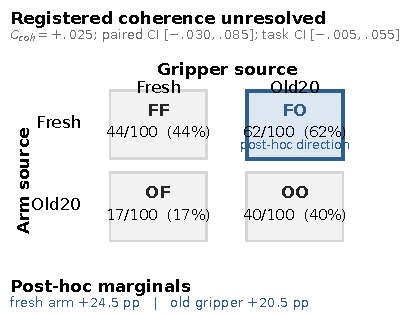
\includegraphics[width=\columnwidth]{fig2_developmental_factorial.pdf}
    \caption{\textbf{Developmental temporal-source factorial.} Cell labels
    give successes from $n=100$ paired task-state blocks per condition. The
    registered coherence contrast compares the mean of FF and OO with the mean
    of FO and OF; its paired-block and task-cluster 95\% bootstrap intervals
    both span zero. The highlighted FO direction and the marginal source
    effects were identified post hoc and used only to define the later
    confirmatory hypothesis.}
    \label{fig:development}
\end{figure}

\subsection{Offline accuracy and closed-loop utility disagree}

At $d=20$, the teacher-forced audit preferred the old source for every measured
component (Fig.~\ref{fig:offline_closedloop}). Normalized translation loss was
.59578 for fresh and .50667 for old; normalized rotation loss was 1.12962 for
fresh and 1.09877 for old. Gripper sign error was .30760 for fresh and .27400
for old. Lower is better for all three metrics. Closed-loop development instead
favored a fresh arm and old gripper.

The disagreement is component-specific: the gripper direction matches across
offline and closed-loop views, while the arm direction reverses. It does not
show that demonstrations are wrong or identify a causal mechanism. It shows
that teacher-forced component prediction accuracy and closed-loop temporal-source
utility are not equivalent objectives in this audited setting. The observed
offline balanced interaction is numerical zero to floating-point tolerance, as
required by Eq.~\eqref{eq:separable_identity}.

\begin{figure}[t]
    \centering
    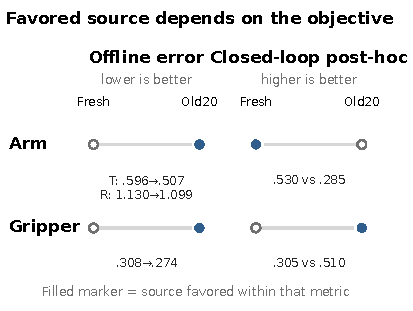
\includegraphics[width=\columnwidth]{fig3_offline_closed_loop.pdf}
    \caption{\textbf{Temporal-source preference depends on the measurement
    objective.} Arrows indicate the favored source rather than placing
    incomparable raw quantities on one axis. Teacher-forced losses over 82
    demonstration episodes and 10,654 eligible targets favor old arm and old
    gripper predictions. Post-hoc closed-loop marginal effects over 100 paired
    task-state blocks favor a fresh arm and old gripper. Lower error is better
    offline; higher success is better closed loop.}
    \label{fig:offline_closedloop}
\end{figure}

\subsection{Asymmetric temporal reuse is confirmed}

FO20 achieved 80/126 successes (63.5\%) on the primary cohort
(Fig.~\ref{fig:confirmation}a). Newest achieved 53/126 (42.1\%), full old20
55/126 (43.7\%), age-exponential ensembling 62/126 (49.2\%), and CogACT 59/126
(46.8\%). Thus FO20 improved over both single-source controls and both shared
full-action temporal-weighting baselines.

All four registered contrasts were stable positive
(Fig.~\ref{fig:confirmation}b). FO20 minus newest was $+.214$, with
paired-block CI $[+.143,+.294]$ and task-cluster CI $[+.127,+.310]$. FO20 minus
full old20 was $+.198$, with intervals $[+.095,+.302]$ and
$[+.063,+.317]$. FO20 minus age-exponential was $+.143$, with intervals
$[+.048,+.238]$ and $[+.016,+.278]$. FO20 minus CogACT was $+.167$, with
intervals $[+.071,+.262]$ and $[+.040,+.294]$. Every leave-one-task-out
estimate was positive for every comparison.

The aggregate result does not imply uniform task-level improvement. Against
full old20, for example, FO20 was lower on one task, tied on one, and higher on
seven. The task-cluster intervals and leave-one-task-out checks explicitly
carry this heterogeneity into the inference. The conclusion is therefore an
aggregate, task-spanning effect for the frozen primary cohort.

\begin{figure*}[t]
    \centering
    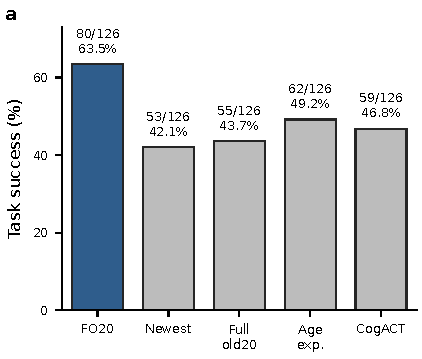
\includegraphics[width=0.38\textwidth]{fig4a_success_rates.pdf}\hfill
    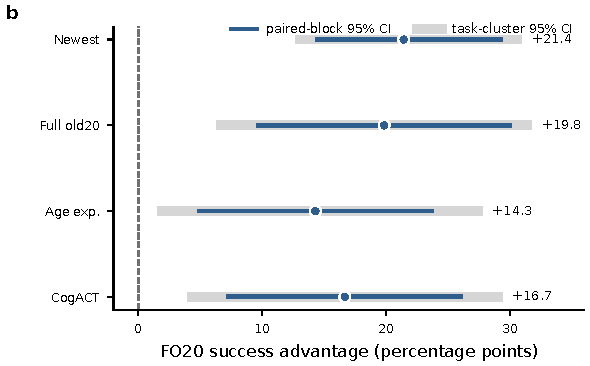
\includegraphics[width=0.56\textwidth]{fig4b_contrasts.pdf}
    \caption{\textbf{Preregistered confirmation on untouched primary states.}
    \textbf{a}, Success counts and rates for the five executors over $n=126$
    paired task-state blocks (nine tasks, 14 states each). \textbf{b}, Four
    registered FO20-minus-comparator success-rate differences. Circles are
    paired estimates; thick and thin intervals are 95\% paired-block and
    task-cluster percentile bootstrap intervals, respectively, each from
    20,000 draws. The dashed line marks no difference. All interval lower
    bounds and every leave-one-task-out estimate are positive.}
    \label{fig:confirmation}
\end{figure*}

\section{Discussion}
\label{sec:discussion}

The confirmatory study establishes a narrow but consequential execution result:
components of one jointly predicted action chunk can benefit from different
observation-time source ages. Because every method observes and queries at the
same controller steps, the result cannot be attributed to different feedback
frequency, query budget, or open-loop horizon. Because newest and full old20
use the same candidate cache, it also cannot be reduced to a general advantage
for fresh or delayed actions. The benefit lies in the asymmetric assignment in
this system.

This conclusion differs from the developmental question. The balanced
factorial did not support a generic incoherence penalty for mixed-source
actions. Its directional cell pattern motivated a new, fixed hypothesis, which
the untouched-state experiment then tested. Keeping that distinction visible
prevents the 62\% developmental FO result from being counted as independent
confirmation.

The result also clarifies how component-aware execution differs from related
work. DAM-VLA already demonstrates that arm and gripper can merit specialized
architectures~\cite{peng2026damvla}; our contribution is not heterogeneity
alone. TRACT routes predicted future behavior across procedural phases and
corrects arm execution~\cite{liu2026tract}; our temporal variable is instead
the past observation that generated a same-time cached prediction. TAS is the
closest source-selection formulation, but selects a complete cached action
~\cite{weng2025tas}. These distinctions make the controlled intervention, not
algorithmic complexity, the main methodological contribution.

The teacher-forced audit cautions against selecting a temporal source from
offline imitation error alone. Old predictions better match demonstrations for
both arm terms, yet the closed-loop factorial favors the fresh arm. Several
explanations are compatible with this mismatch: fresh feedback may correct
state deviation, demonstrations may reward temporal consistency differently
from the closed loop, or the separable metric may omit behaviorally important
coupling. The experiments do not distinguish these explanations. In
particular, they do not prove retained intent, non-Markovian causation, or any
general temporal-intent mechanism.

FO20 is deliberately simple. It adds no training, estimator, or policy head,
and its result suggests a future adaptive executor could predict source utility
per component. Such adaptation is not evaluated here. A learned rule would
need an independent cohort and should be compared under the same current-
observation and matched-query contract.

\subsection{Limitations}

The evidence uses one frozen ACT checkpoint and the LIBERO Object suite. It
tests one six-dimensional arm/scalar-gripper partition and confirms one source
gap, $d=20$. The study neither proves that 20 ticks is optimal nor evaluates
dynamic adaptation. It provides no causal proof that an old gripper prediction
retains intent or that non-Markovian structure produces the success gain.
There is no current confirmation on a second policy, another benchmark, a VLA,
a dexterous or bimanual action space, or a real robot. The primary cohort spans
nine tasks and paired unused states, which supports within-system credibility
but not broad generalization. Finally, success is binary; logged kinematic and
disagreement diagnostics follow treatment-dependent trajectories and are not
used to make mechanistic claims.

\section{Conclusion}
\label{sec:conclusion}

Repeated action-chunk queries provide multiple observation-conditioned
predictions for the same physical time. In one frozen ACT/LIBERO Object system,
assigning the fresh source to arm motion and the 1.0-s-old source to the gripper
improved success over four full-action execution rules under identical
observation access and query cadence. The result confirms that temporal-source
age need not be shared across heterogeneous components of a jointly predicted
action. At the same time, the offline audit shows that separable imitation
accuracy can select a different source and cannot represent the symmetric
component interaction. Component-specific temporal reuse is therefore a
distinct execution variable that should be evaluated in closed loop, with its
generality tested rather than assumed.


\section*{Acknowledgment}
OpenAI Codex assisted with manuscript drafting, editing, and figure-code
development. The authors verified the numerical claims, citations, and final
artifacts against the frozen project records.

\bibliographystyle{IEEEtran}
\bibliography{references}

\end{document}
